%%%%%%%%%%%%%%%%%%%%%%%%%%%%%%%%%%%%%%%%%%%%%%%%%%%%%%%%%%%%%%%%%%%%%%%%%%%%%%%%
%2345678901234567890123456789012345678901234567890123456789012345678901234567890
%        1         2         3         4         5         6         7         8


\documentclass[letterpaper, 10 pt, conference]{ieeeconf}  % Comment this line out
                                                          % if you need a4paper
%\documentclass[a4paper, 10pt, conference]{ieeeconf}      % Use this line for a4
                                                          % paper

\IEEEoverridecommandlockouts                              % This command is only
                                                          % needed if you want to
                                                          % use the \thanks command
\overrideIEEEmargins
% See the \addtolength command later in the file to balance the column lengths
% on the last page of the document

\usepackage{graphicx}
\usepackage{float}
\usepackage{graphics}
\usepackage[utf8]{inputenc}
%\usepackage[spanish, activeaccute]{babel} %permite escribir con ortografía en español, acentos, ñ, etc
\usepackage[spanish,es-noshorthands]{babel}
\usepackage{mathtools} %matematica
\usepackage{amsmath} %matematica
\usepackage{circuitikz} %pa dibujar circuitoz
\usepackage{siunitx} %simbologia, ohm etc
\usepackage{amssymb}
\usepackage{hyperref}


% Para los acentos
%\usepackage[spanish]{babel}
% The following packages can be found on http:\\www.ctan.org
%\usepackage{graphics} % for pdf, bitmapped graphics files
%\usepackage{epsfig} % for postscript graphics files
%\usepackage{mathptmx} % assumes new font selection scheme installed
%\usepackage{times} % assumes new font selection scheme installed
%\usepackage{amsmath} % assumes amsmath package installed
%\usepackage{amssymb}  % assumes amsmath package installed

\title{\LARGE \bf
Laboratorio 3 - Circuitos Electrónicos I - Ing. Electrónica
}

%\author{ \parbox{3 in}{\centering Huibert Kwakernaak*
%         \thanks{*Use the $\backslash$thanks command to put information here}\\
%         Faculty of Electrical Engineering, Mathematics and Computer Science\\
%         University of Twente\\
%         7500 AE Enschede, The Netherlands\\
%         {\tt\small h.kwakernaak@autsubmit.com}}
%         \hspace*{ 0.5 in}
%         \parbox{3 in}{ \centering Pradeep Misra**
%         \thanks{**The footnote marks may be inserted manually}\\
%        Department of Electrical Engineering \\
%         Wright State University\\
%         Dayton, OH 45435, USA\\
%         {\tt\small pmisra@cs.wright.edu}}
%}

\author{Ignacio Nahuel Chantiri 69869/1 \\  %\vspace{1cm}
{\it Universidad Nacional De La Plata, Argentina,}
{\it Junio 2024.}}                              % <-this % stops a space

\begin{document}


\maketitle
\thispagestyle{empty}
\pagestyle{empty}


%%%%%%%%%%%%%%%%%%%%%%%%%%%%%%%%%%%%%%%%%%%%%%%%%%%%%%%%%%%%%%%%%%%%%%%%%%%%%%%%
\begin{abstract}

El análisis de laboratorio presentado describe el estudio del efecto de la realimentación de un amplificador de múltiples etapas, y el análisis del comportamiento de cascada de dichas etapas de transitores BJT.\\
\end{abstract}


%%%%%%%%%%%%%%%%%%%%%%%%%%%%%%%%%%%%%%%%%%%%%%%%%%%%%%%%%%%%%%%%%%%%%%%%%%%%%%%%
\section{Introducci\'on}

El informe posee el siguiente formato:\\
Primeramente, incluye un \textit{Marco Teórico} que abarca las explicaciones y describe el comportamiento esperado.\\ A continuación, se presenta el \textit{Desarrollo experimental}, con la descripción del set-up y conexiones de la placa, junto con los resultados y mediciones correspondientes, seguido finalmente de una conclusión y comparación con las cuentas analíticas para cada uno de los pasos realizados.


\section{Marco teórico}



\subsection{\textbf{Etapa amplificadora con transistor BJT con emisor común.}}

El circuito está compuesto por tres etapas de emisor común. A continuación se analizará la ganancia de una, y su capacidad de acoplarse según su impedancia de entrada y de salida.\\
En la \textit{Figura 1} se presenta el diagrama circuital de una etapa individual:

\begin{figure}[H]
  \centering
  \begin{circuitikz}
    \node[npn] (npn) at (0,0) {};
    \draw (npn.base) -- ++(-1, 0) -- ++(0, -1) to[R=$\qty{39}{\kilo\ohm}$] ++(0, -1.5) -- ++(0, -0.5) node[ground]{};
    \draw (npn.base) -- ++(-1, 0) -- ++(0, 1.5) to[R=$\qty{100}{\kilo\ohm}$] ++(0, 1.5) -- ++(0, 0.5) node[ocirc]{} coordinate (Vp) node[right, font=\large] {$+V$}; 
    \draw (npn.collector) -- ++(0, 0.75) to[R=$\qty{560}{\ohm}$] ++(0, 1.5) -- ++(0, 0.5) node[ocirc]{} coordinate (Vp) node[right, font=\large] {$+V$};
    % TODO: buscar el simbolo de pico para los faradios
    \draw (npn.collector) -- ++(0, 0.5) node[circ]{} -- ++(-0.75, 0) to[C=$\qty{10}{\pico\farad}$] ++(-0.5, 0) -- ++(-0.6, 0) node[circ]{};
    \draw (npn.collector) node[circ]{} -- ++(1, 0) to[C=$\qty{10}{\micro\farad}$] ++(1, 0) -- ++(0.75, 0) node[ocirc]{} coordinate (Vin) node[right, font=\large] {$V_{s}$};
    \draw (npn.emitter) -- ++(0, -0.25) to[R=$\qty{100}{\ohm}$] ++(0, -1.5) -- ++(0, -0.5) node[ground]{};
    \draw (npn.base) -- ++(-1, 0) node[circ]{} -- ++(-1, 0) to[C=$\qty{10}{\micro\farad}$] ++(-1, 0) -- ++(-0.75, 0) node[ocirc]{} coordinate (Vin) node[left, font=\large] {$V_{i}$};
  \end{circuitikz}
  \caption{Transistor NPN en configuración de Emisor Común.}
  \label{fig:etapaemisorcomun}
\end{figure}

\subsubsection{Ganancia de Tensión $Av$ de una etapa individual (etapas 1 y 2).}

Del modelo de pequeña señal, y aproximando la corriente del Emisor como $gmV_{\pi}$, se obtiene el siguiente sistema de ecuaciones:

\begin{equation}
\left\{
\begin{aligned}
V_o &= -g_m V_{\pi}R_C \\ 
V_{\pi} &= V_i - V_{R_e} \Longrightarrow V_i = V_{\pi}(gmR_e + 1)\\
\end{aligned}
\right.
\end{equation}

Por lo que la ganancia $Av = \frac{V_o}{V_i}$, considerando el producto $gmR_e >> 1$, será:

\begin{equation}
Av_{1,2} = \frac{-gmR_c}{gmR_e+1} \approx -\frac{R_c}{R_e}
\end{equation}

Para el caso particular de estudio con valores $R_c = 560\Omega$ y $R_e = 100\Omega$, la ganancia de tensión de la etapa individual 1 y 2 es:

\begin{equation}
Av_{1,2} \approx -\frac{560\Omega}{100\Omega} \approx -5,6 \\[1em]
\end{equation}

\subsubsection{Impedancia de entrada $Z_{in}$}

\begin{equation}
\\[1em]Z_{in} = R_1//R_2 = \frac{100k\Omega 39k\Omega}{100k\Omega + 39k\Omega} \approx 28k\Omega
\label{eq:zin_individual}
\end{equation}

\subsubsection{Impedancia de salida $Z_{out}$}

\begin{equation}
Z_{out} = R_c = 560\Omega
\label{eq:zout_individual}
\end{equation}

\subsubsection{Ganancia de Tensión $Av$ de la última etapa}
La salida de la útlima etapa se ve cargada por un resistor de $1k\Omega$. La ganancia se obtiene de igual manera que las etapas anteriores, pero la carga será el resistor del colector $R_c$ ahora en paralelo con el resistor de $1k\Omega$:

\begin{equation}
Av_3 \approx -\frac{R_c//1k\Omega}{R_e} \approx -3,58
\end{equation}

\subsection{\textbf{Amplificador Multietapa a Lazo Abierto.}}
El circuito a utilizar consta de tres etapas en cascada de transistores BJT NPN idénticas a las analizadas en la sección previa. Se analizarpa primeramente el Lazo Abierto.\\

En la figura a continuación se presenta un diagrama circuital de la placa utilizada:

\begin{figure}[H]
  \centering
  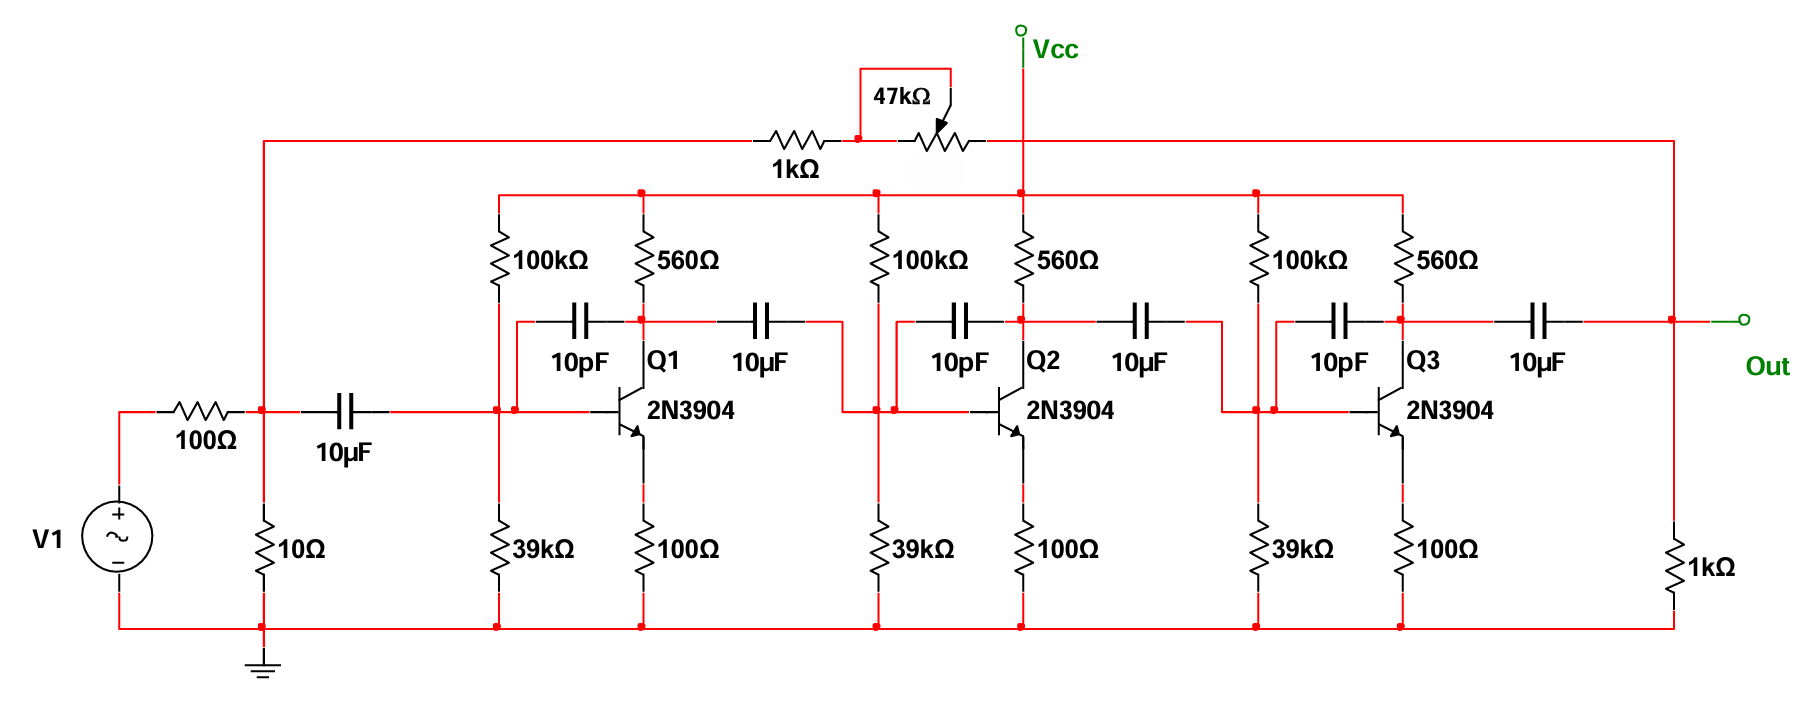
\includegraphics[width=0.47\textwidth]{imagenes/diagrama placa.png}
  \caption{Diagrama circuital de la placa utilizada.}
  \label{fig:diagramaplaca}
\end{figure}

\subsubsection{Ganancia de Tensión $Av_{LA}$ Multietapa a Lazo Abierto}

En la sección previa se verificó que cada etapa individual presenta una alta impedancia de entrada y una baja impedancia de salida, de modo que puede considerarse que las tres etapas en cascada se acoplan tal que la ganancia total es el producto de las ganancias de cada etapa:

\begin{equation}
Av_{LA} \approx Av_1  Av_2  Av_3 \approx (-5,6)(-5,6)(-3,58)
\end{equation}

\begin{equation}
Av_{LA} \approx -112,26
\end{equation}

\subsubsection{Impedancia de entrada del Amplificador Multietapa a Lazo Abierto $Z_{in}$}

La impedancia de entrada será la misma que la de la primer etapa individual. De \ref{eq:zin_individual}:

\begin{equation}
Z_{in} \approx 28k\Omega 
\end{equation}

\subsubsection{Impedancia de salida del Amplificador Multietapa a Lazo Abierto $Z_{out}$}\\

La impedancia de salida será la misma que la de la última etapa individual.  De \ref{eq:zout_individual}:

\begin{equation}
Z_{out} = 560\Omega
\end{equation}

\subsubsection{Ganancia de Transimpedancia $Az_{LA}$ Multietapa a Lazo Abierto}

Para el análisis posterior sobre realimentación, resulta de interés convertir la ganancia $Av_{LA}$ en una ganancia de Transimpedancia $Az_{LA} =\frac{V_o}{I_i}$. Esto se logra reescribiendo la tensión de entrada $V_o$ en función de la corriente de entrada $I_i$, obteniendo:

\begin{equation}
Az_{LA} = Av_{LA} . Z{in} = (-112,26)28k\Omega
\end{equation}

\begin{equation}
Az_{LA}  -3,14M\frac{V}{A}
\end{equation}

\subsection{\textbf{Amplificador multietapa Realimentado.}}

La realimentación se da por una rama desde la entrada de la primer etapa a la salida de la última, compuesta por un bloque beta que contiene un resistor y un potenciómetro en serie, de manera tal que se pueda variar la resistencia del bloque Beta entre y $1k\Omega$ y $48k\Omega$.\\
Es por ello que el análisis a continuación describe ecuaciones pero no incluye los valores numéricos obtenidos, sino que se muestran posteriormente en la \textit{Tabla I} en la sección \textit{II-D}, para una mayor prolijidad.

\subsubsection{Ganancia de Tensión $Az_{cargado}$}

Para obtener la ganancia final del cirucito realimentado, se precisa conocer primero la ganancia $A_{cargado}$, correspondiente al bloque $A$ cargado con el bloque $\beta$.\\
La topología que presenta es Paralelo-Paralelo, que corresponde a un amplificador de Transimpedancia, diagramada en la siguiente figura:

\begin{figure}[H]
  \centering
  \begin{circuitikz}

    % bloque de lazo directo
    \node (square) [draw,minimum width=2cm,minimum height=2cm,anchor=south west] at (0,0) {a};
    \draw (square.west) |- ++(-2, 0.5) node[ocirc]{};
    \draw (square.west) |- ++(-2, -0.5) node[ocirc]{};
    \draw (square.east) |- ++(2, 0.5) node[ocirc]{};
    \draw (square.east) |- ++(2, -0.5) node[ocirc]{};

    % bloque de realimentación
    \node (square_b) [draw,minimum width=1.5cm,minimum height=1.5cm,anchor=south west] at (0.25, -2) {$\beta$};
    \draw (square_b.west) |- ++(-0.75, 0.5) -- ++(0, 2.25) node[circ]{};
    \draw (square_b.west) |- ++(-1.25, -0.5) -- ++(0, 2.25) node[circ]{};
    \draw (square_b.east) |- ++(0.75, 0.5) -- ++(0, 2.25) node[circ]{};
    \draw (square_b.east) |- ++(1.25, -0.5) -- ++(0, 2.25) node[circ]{};

  \end{circuitikz}
  \caption{Topología Paralelo-Paralelo correspondiente a un circuito amplificador de Transimpedancia.}
  \label{diag:transimpedancia}
\end{figure}

Siendo el bloque Beta:

\begin{figure}[H]
  \centering
  \begin{circuitikz}

    % bloque de lazo directo
    \node (square) [draw,minimum width=4cm,minimum height=3.5cm,anchor=south west] at (0,0) {$\beta$};
    \draw (square.west) ++(-1, 0.75) node[ocirc]{} -- ++(1.5, 0) to[R=\qty{1}{\kilo\ohm}] ++(1.25, 0) to[vR=\qty{47}{\kilo\ohm}] ++(2,0) -- ++(1,0) -- ++(0.25,0) node[ocirc]{};
    \draw (square.west) ++(-1, -0.75) node[ocirc]{} -- ++(6,0) node[ocirc]{};
  \end{circuitikz}
  \caption{Bloque beta de realimentación}
  \label{diag:bloque_beta}
\end{figure}

Donde el bloque Beta posee los valores de transferencia de transadmitancia $\beta$, admitancia de entrada $y_{i\beta}$ y admitancia de salida $y_{o\beta}$ representados por los parámetros $Y$ listados a continuación:

\begin{equation}
\begin{aligned}
\beta &= y_{12} = \frac{I_1}{U_2} \bigg\rvert_{U_1 = 0} = -\frac{1}{R_f} \\[1em]
y_{i\beta} &= y_{11} = \frac{I_1}{U_1} \bigg\rvert_{U_2 = 0} = \frac{1}{R_f}\\[1em]
y_{o\beta} &= y_{22} = \frac{I_2}{U_2} \bigg\rvert_{U_1 = 0} = \frac{1}{R_f}\\
\end{aligned}
\label{eq:parametrosbeta}
\end{equation}

Con $R_f = 1k\Omega + R_p$ ($R_p$ siendo la resistencia variable del potenciómetro).\\
Incluyendo $y_{11}^{-1}$ y $y_{22}^{-1}$ dentro del bloque A, se obtiene la ganancia de transimpedancia del bloque \textit{A} cargado:

\begin{figure}[H]
  \centering
  \scalebox{0.7}{
  \begin{circuitikz}

    % bloque de lazo directo
    \draw (0,0) node[ocirc]{} coordinate (Vp) node[left, font=\large] {$V_i$ $+$} -- ++(0.25, 0) to[short, f>^=$I_i$] ++(0.75, 0) node[circ]{} -- ++(0, 0) to[R, l_=$y_{11}^{-1}$] ++(0, -2) node[circ]{} -- ++(-1, 0) node[ocirc]{} coordinate (Vp) node[left, font=\large] {$-$};
    \draw (0,0) -- ++(2.5,0) to[R, l_= $Z_{in}$, f>^=$I_{a}$] ++(0, -2) -- ++(-2.5, 0);
    \draw (0,0) ++(4,0) -- ++(0,0) to[american controlled voltage source, l=$Az_{LA}.I_{a}$] ++(0, -2);
    \draw (0,0) ++(4,0) -- ++(1, 0) to[R=$Z_{out}$] ++(1.5, 0) -- ++(1, 0) node[circ]{} -- ++(1,0) node[ocirc]{} coordinate (Vp) node[right, font=\large] {$+$ $V_o$};
    \draw (0,0) ++(7.5,0) to[R=$y_{22}^{-1}$] ++(0, -2) -- ++(-3.5, 0) ++(3.5, 0) node[circ]{} -- ++(1, 0) node[ocirc]{} coordinate (Vp) node[right, font=\large] {$-$};

  \end{circuitikz}
  }
  \caption{Bloque A cargado.}
  \label{fig:diagrama_bloques_realimentacion}
\end{figure}

$Az_{cargado} = \frac{V_o}{I_i}$ se deriva planteando el siguiente sistema de ecuaciones:

\begin{equation}
\left\{
\begin{aligned}
V_o &= \frac{Az_{LA} I_a y_{22}^{-1}}{y_{22}^{-1}+Z_{out}} \\ 
I_a &= \frac{I_i}{Z_{in}(y_{11}+Z_{in}^{-1})}\\
\end{aligned}
\right.
\end{equation}
Resulta:
\begin{equation}
Az_{cargado} = \frac{V_o}{I_i} =  \frac{Az_{LA}}{(1+Z_{out}y_{22})(y_{11}Z_{in}+1)}\\[1em]
\label{eq:azcargado}
\end{equation}

\subsubsection{Ganancia de Transimpedancia $Az_r$ del circuito realimentado}

Para obtener la ganancia de Tensión $Av_r$ del circuito realimentado, nos valemos de la siguiente fórmula:

\begin{equation}
Az_r = \frac{Az_{cargado}}{1+\beta Az_{cargado}}
\label{eq:azr}
\end{equation}

Donde $Az_{cargado}$ corresponde a la ganancia del bloque $A$ cargado con el bloque $\beta$, mientras que $\beta$ es la transferencia $\frac{I_1}{V_2}$ del bloque de realimentación, ambas obtenidas en la sección anterior.\\

\subsubsection{Impedancia de entrada $Zin_{r}$ del circuito realimentado}

La impedancia de entrada (del bloque A cargado) disminuye al realimentar, por un factor de $1+\beta Az_{cargado}$:

\begin{equation}
Zin_r = \frac{y_{11}^{-1}Z_{in}}{y_{11}^{-1}+Z_{in}}\frac{1}{1+\beta Az_{cargado}}\\[em]
\label{eq:zinr}
\end{equation}

El termino en paralelo corresponde a la impedancia de entrada para el bloque A cargado, siendo $Z_{in}$ la impedancia de entrada del mismo bloque pero sin cargar, y $y_{11}^{-1}$ la impedancia de entrada del bloque Beta\\

\subsubsection{Ganancia de Tensión $Av_r$ del circuito realimentado}

En el desarrollo del laboratorio se pretende medir ganancia de tensión del circuito completo. Es por ello que es preferible transformar la ganancia de transimpedancia $Az_r$ a una ganancia de tensión $Av_r = \frac{V_o}{V_i}$:

\begin{equation}
I_i = \frac{V_i}{Zin_r}\\[em]
\end{equation}

Reemplazando en $Az_r = \frac{V_o}{I_i}$:

\begin{equation}
 Az_r = \frac{V_o}{V_i} Zin_r = Av_rZin_r \\
\end{equation}

\begin{equation}
\therefore Av_r = \frac{Az_r}{Zin_r}
\label{eq:avr}
\end{equation}

\subsection{\textbf{Valores extremos}}
Recordemos que la resistencia $R_f$ de la rama de realimentación está compuesta por un potenciómetro, que permite fijar en la rama un valor de resistencia entre $1k\Omega$ y $48k\Omega$.\\
A continuación se presentan en forma de tabla los valores numéricos de los parámetros obtenidos en esta sección, para las resistencias extremas de realimentación:


\begin{table}[h]
\begin{center}
\begin{tabular}{|c||c|c|c|}
\hline
Parámetro & Ecuación & $R_f = 1k\Omega$ & $R_f = 48k\Omega$\\
\hline
$\beta$ & \ref{eq:parametrosbeta} & -$1m \frac{A}{V}$ & $-20,83\mu \frac{A}{V}$\\
\hline
$y_{i\beta}$ & \ref{eq:parametrosbeta} & $1 mS$ & $20,83\mu S$\\
\hline
$y_{o\beta}$ & \ref{eq:parametrosbeta} & $1 mS$ & $20,83\mu S$\\
\hline
$Az_{cargado}$ & \ref{eq:azcargado} & $-69.
4k\frac{V}{A}$ & $-1.73M\frac{V}{A}$\\
\hline
$Zin_r$ & \ref{eq:zinr} & $14\Omega$ & $316\Omega$\\
\hline
$Az_r$ & \ref{eq:azr} & $-985,8 \frac{V}{A}$ & $-34,9k\frac{V}{A}$\\
\hline
$Av_r$ & \ref{eq:avr} & $-71,9$ & $-110,5$\\
\hline
$Av_{total}$ &  & $-3,9$ & $-9,7$\\
\hline
\end{tabular}
\end{center}
\caption{Parámetros del amplificador, para casos extremos de $R_f$.}
\label{tab:parametros}
\end{table}

Donde $Av_{total}$ es la ganancia que se medirá en el laboratorio, ya que considera el divisor de tensión de la entrada de la placa.

\section{Desarrollo experimental}
Se describirán a continuación las mediciones hechas y los resultados obtenidos.\\
La placa consiste en un amplificador multietapa realimentado, como el estudiado en la sección del Marco Teórico.\\
Se propuso entonces medir dos factores: la ganancia de tensión realimentada; y el ancho de banda, ambos para los valores extremos de las resistencias de realimentación del bloque beta.

\subsection{\textbf{Conexiones y consideraciones para la medición}}

\begin{itemize}
  \item Se administró una tensión continua de polarización de $12V$,
  \item Se conectó un generador de funciones a la entrada, entre los terminales 'E' y tierra. La función suministrada será siempre una onda senoidal de amplitud $200mV$,
  \item Se conectó un osciloscopio a la entrada y a la salida, quedando representadas siempre la entrada en color amarillo, y la salida en azul.
\end{itemize}

\begin{figure}[H]
  \centering
  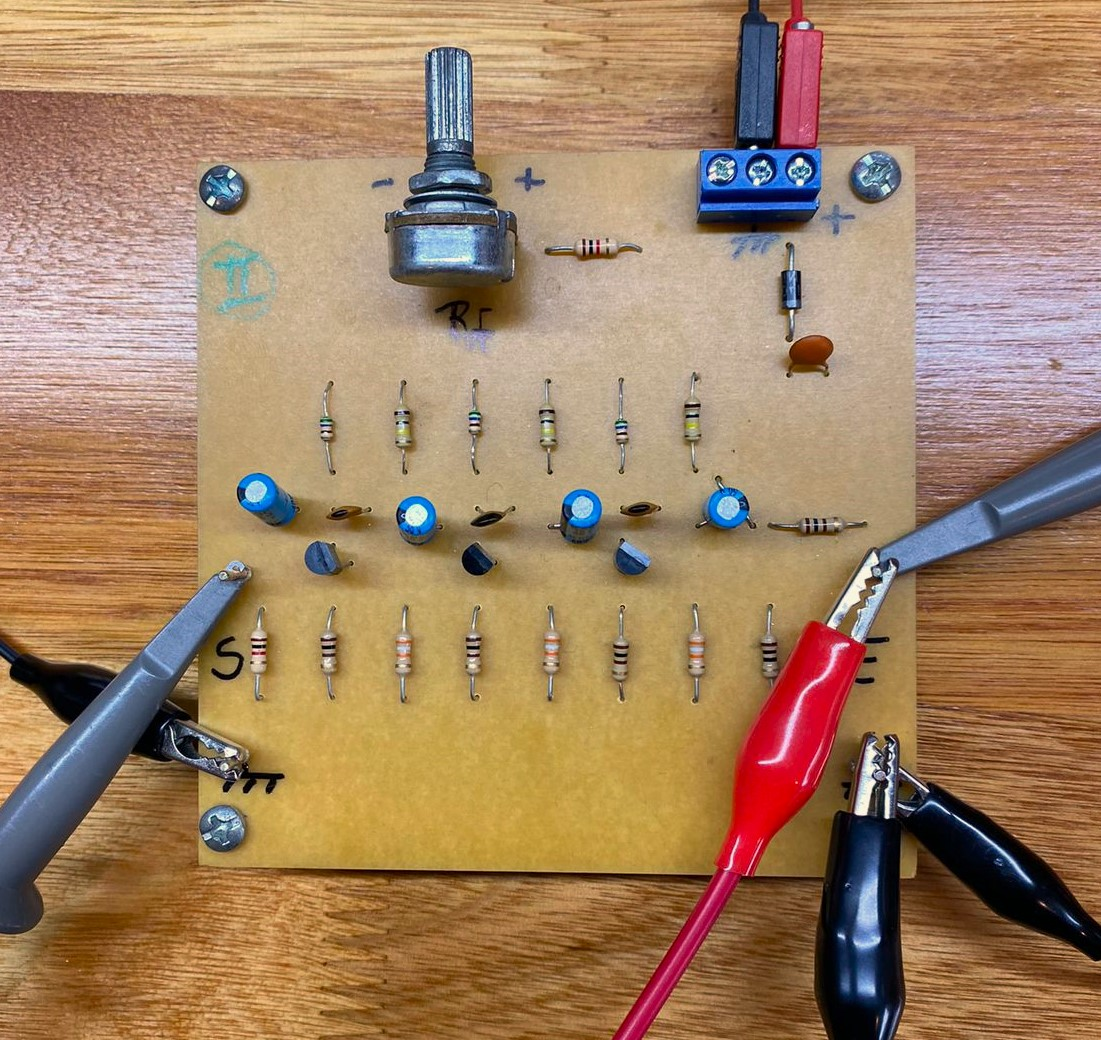
\includegraphics[width=0.47\textwidth]{imagenes/placa conectada.jpg}
  \caption{Conexión final de los instrumentos a la placa}
  \label{fig:placaconectada}
\end{figure}

\subsection{\textbf{Ganancia de Tensión Realimentada $Av_r$}}

Se pocedió entonces a la medición de la Ganancia de Tensión con el circuito realimentado, inyectando una señal senoidal de amplitud $200mV$ y frecuencia $10kHz$.
La frecuencia elegida se consideró lo suficientemente baja como para no verse afectada por el polo dominante del circuito.\\

\subsubsection{Potenciómetro en mínimo}

Primeramente, se dispuso el potenciómetro en mínimo ($0\Omega$), quedando el bloque Beta compuesto solo por la resistencia de $1k\Omega$.
Para la entrada de $200mV$, se midió una salida de $950mV$, correspondiente a una ganancia $Av_r = -4,75$. Esto da un error relativo del $20,6\%$ comparado al valor teórico calculado.\\[em]

\subsubsection{Potenciómetro en máximo}

A continuación, se subió el potenciómetro a su valor máximo ($47k\Omega$), quedando el bloque Beta como una resistencia de $48k\Omega$.
Para la entrada de $200mV$, se midió una salida de $1,8V$, correspondiente a una ganancia $Av_r = -9$. Esto da un error relativo del $7,2\%$ comparado al valor teórico calculado.\\[em]

\begin{table}[h]
\begin{center}
\begin{tabular}{|c||c|c|}
\hline
 & $R_f = 1k\Omega$ (mín.) & $R_f = 48k\Omega$ (máx.) \\
\hline
Entrada [$mV$] & $200$ & $200$ \\
\hline
Salida [$mV$] & $950$ & $1800$ \\
\hline
$Av_r medida$ & $-4,75$ & $-9$ \\
\hline
$Av_r teórica$ & $-3,9$ & $-9,7$ \\
\hline
Error Relativo & $20,6\%$ & $7,2\%$ \\
\hline
\end{tabular}
\end{center}
\caption{Mediciones de Ganancia}
\label{tab:simple}
\end{table}


Las ganancias medidas se asemejan a lo esperado, pero igualmente el error obtenido del $20\%$ para la primer medición es mayor a lo deseado.

\subsection{\textbf{Ancho de banda}}

Para estudiar el ancho de banda se realizó un barrido de frecuencia desde $10k\Omega$ hasta medir en la salida una atenuación de $3dB$.\\[em]

\subsubsection{Potenciómetro en mínimo}
Para el potenciómetro en mínimo se obtuvo previamente una salida de $950mV$, por lo que su polo estará ubicado donde se produzca una atenuación de $3dB$, es decir, cuando su valor de salida sea $\frac{950mV}{\sqrt{2}} = 671,7mV$\\
Se realizó el barrido de frecuencia y se halló dicha atenuación a una frecuencia de $840kHz$.\\[em]

\subsubsection{Potenciómetro en mínimo}
Para el potenciómetro en mínimo se obtuvo previamente una salida de $1,8V$, por lo que su polo estará ubicado donde se produzca una atenuación de $3dB$, es decir, cuando su valor de salida sea $\frac{1,8V}{\sqrt{2}} = 1,27V$\\
Se realizó el barrido de frecuencia y se halló dicha atenuación a una frecuencia de $1,57MHz$.\\[em]

Las mediciones de frecuencia no son las esperadas, pues el producto ganancia x ancho de banda no se mantuvo.

\begin{table}[h]
\begin{center}
\begin{tabular}{|c||c|}
\hline
Resistencia Bloque Beta & Frecuencia de corte\\
\hline
$1k\Omega$ (mín.) & 840kHz\\
\hline
$48k\Omega$ (máx.) & 1,57MHz\\
\hline
\end{tabular}
\end{center}
\caption{Frecuencias de corte $(3dB)$}
\label{tab:simple}
\end{table}

\section{Conclusiones}

Debido a varias complicaciones durante el laboratorio, las imágenes tomadas mostraban mediciones mal hechas, por lo que no se incluyeron en el informe. Además, no se logró ubicar los polos de manera satisfactoria, y tampoco se obtuvieron los valores teóricos esperados para las ganancias. No logramos estimar el porqué de las diferencias entre los valores esperados y los medidos.
 

\addtolength{\textheight}{-12cm}   % This command serves to balance the column lengths
                                  % on the last page of the document manually. It shortens
                                  % the textheight of the last page by a suitable amount.
                                  % This command does not take effect until the next page
                                  % so it should come on the page before the last. Make
                                  % sure that you do not shorten the textheight too much.

%%%%%%%%%%%%%%%%%%%%%%%%%%%%%%%%%%%%%%%%%%%%%%%%%%%%%%%%%%%%%%%%%%%%%%%%%%%%%%%%



%%%%%%%%%%%%%%%%%%%%%%%%%%%%%%%%%%%%%%%%%%%%%%%%%%%%%%%%%%%%%%%%%%%%%%%%%%%%%%%%



%%%%%%%%%%%%%%%%%%%%%%%%%%%%%%%%%%%%%%%%%%%%%%%%%%%%%%%%%%%%%%%%%%%%%%%%%%%%%%%%



%\section*{ACKNOWLEDGMENT}

%The preferred spelling of the word Òacknowledgment\'o in America is without an Òe\'o after the Òg\'o. Avoid the stilted expression, ÒOne of us (R. B. G.) thanks . . .\'o  Instead, try ÒR. B. G. thanks\'o. Put sponsor acknowledgments in the unnumbered footnote on the first page.



%%%%%%%%%%%%%%%%%%%%%%%%%%%%%%%%%%%%%%%%%%%%%%%%%%%%%%%%%%%%%%%%%%%%%%%%%%%%%%%%


\begin{thebibliography}{99}

\bibitem{c1} J. Millman and A. Grabel, ``Microelectrónica,” McGraw-Hill, New York, 6ta edición, 1993.
\bibitem{c2} P. R. Gray and R. G. Meyer, ``Analysis and Design of Analog Integrated Circuits,” John Wiley & Sons, New York, 4th edition, 2001



\end{thebibliography}




\end{document}
